\documentclass[a4paper, 12pt]{article}

\usepackage[T1]{fontenc}
\usepackage{amssymb}
\usepackage{float}
\usepackage{booktabs}

\let\emptyset\varnothing

\usepackage{tikz}
\usetikzlibrary{positioning}

\tikzset{state/.style = {draw, circle, thick, minimum size=0.7cm}}
\tikzset{accepting/.style = {draw, circle, thick, minimum size=0.7cm, double, double distance = 2pt}}
\tikzset{set/.style = {}}
\tikzset{acceptingset/.style = {draw, rectangle, thick}}
\tikzset{starting/.style = {pin={[pin edge={<-, semithick, black}] above left:}}}

\begin{document}

\title{
  Języki Formalne i Techniki Translacji \\
  \vspace{0.5em}
  \begin{center}\Large Lista 1, Zadanie 3\end{center}}
\author{Piotr Kocia}
\maketitle

\tableofcontents

\section{Regular Expression $10 + (0 + 11) 0^{*} 1$}

The regular expression $10 + (0 + 11) 0^{*} 1$ may have its corresponding FA
constructed in a few steps by iteratively lowering its subexpressions. Firstly,
we start with an automaton that has only one transition matching the whole
expression.

\begin{center}
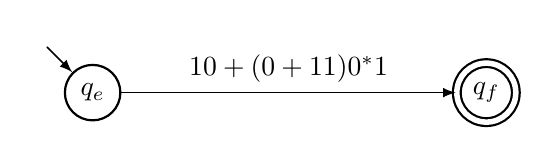
\begin{tikzpicture}[auto, >=latex, on grid, semithick]
  \node [state, starting] (qe) {$q_e$};
  \node [accepting, right=5cm of qe] (qf) {$q_f$};
  \path[->] (qe) edge node[above] {$10 + (0 + 11) 0^{*} 1$} (qf);
\end{tikzpicture}
\end{center}

We separate the expressions at the alternative and create two transitions from
$q_e$ to $q_f$.

\begin{center}
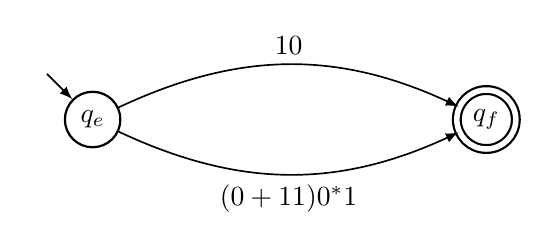
\begin{tikzpicture}[auto, >=latex, on grid, semithick]
  \node [state, starting] (qe) {$q_e$};
  \node [accepting, right=5cm of qe] (qf) {$q_f$};
  \path[->] (qe) edge [bend left=25] node [above] {$10$} (qf);
  \path[->] (qe) edge [bend right=25] node [below] {$(0 + 11) 0^{*} 1$} (qf);
\end{tikzpicture}
\end{center}

Concatenations are sequence events, hence we create sequences of nodes with
transitions inbetween corresponding to the atomic expressions of the
concatenation.

\begin{center}
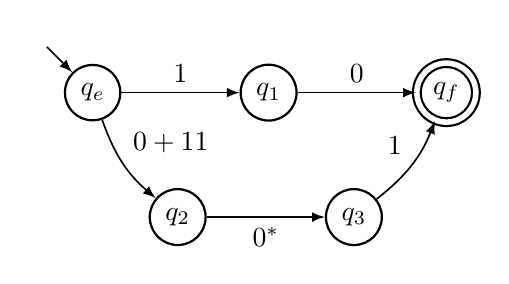
\begin{tikzpicture}[auto, >=latex, node distance=1.5cm, semithick]
  \node [state, starting] (qe) {$q_e$};
  \node [state, right=of qe] (q1) {$q_1$};
  \node [state, below right=of qe, xshift=-0.5cm] (q2) {$q_2$};
  \node [state, right=of q2] (q3) {$q_3$};
  \node [accepting, right=of q1] (qf) {$q_f$};

  \path[->] (qe) edge node [above] {$1$} (q1);
  \path[->] (q1) edge node [above] {$0$} (qf);

  \path[->] (qe) edge [bend right=15] node {$0 + 11$} (q2);
  \path[->] (q2) edge node [below] {$0^{*}$} (q3);
  \path[->] (q3) edge [bend right=15] node {$1$} (qf);
\end{tikzpicture}
\end{center}

The tricky part in this step is the transition with Kleene star. One possible
solution is to create a state that loops to itself on the expression that Kleene
star operates on and provide $\epsilon$ transtions to and from that state.

\begin{center}
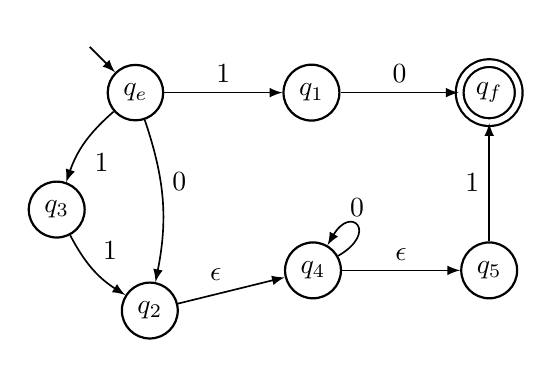
\begin{tikzpicture}[auto, >=latex, node distance=1.5cm, semithick]
  \node [state] (q1) {$q_1$};
  \node [state, starting, left=of q1] (qe) {$q_e$};z
  \node [state, below=of qe, xshift=-1cm, yshift=0.75cm] (q3) {$q_3$};
  \node [state, below right=of q3, xshift=-0.4cm, yshift=0.3cm] (q2) {$q_2$};
  \node [accepting, right=of q1] (qf) {$q_f$};
  \node [state, below=of qf] (q5) {$q_5$};
  \node [state, left=of q5] (q4) {$q_4$};

  \path[->] (qe) edge node {$1$} (q1);
  \path[->] (q1) edge node {$0$} (qf);

  \path[->] (qe) edge [bend left=15] node {$0$} (q2);
  \path[->] (qe) edge [bend right=15] node {$1$} (q3);

  \path[->] (q3) edge [bend right=15] node {$1$} (q2);

  \path[->] (q2) edge node {$\epsilon$} (q4);
  \path[->] (q4) edge [loop, out=30, in=60, looseness=8] node [above] {$0$} (q4);
  \path[->] (q4) edge node {$\epsilon$} (q5);

  \path[->] (q5) edge node {$1$} (qf);
\end{tikzpicture}
\end{center}

At this point we have transformed the entire RE into states and transitions on
the elements of the alphabet, hence what remains is simplification and
elimination of $\epsilon$ transitions. We note that we have a chain of
$\epsilon$ transitions between $q_2$ and $q_5$ with no transitions apart from
the loop in $q_4$. We may simplify that by merging both $q_4$ and $q_5$ into
$q_2$.

\begin{center}
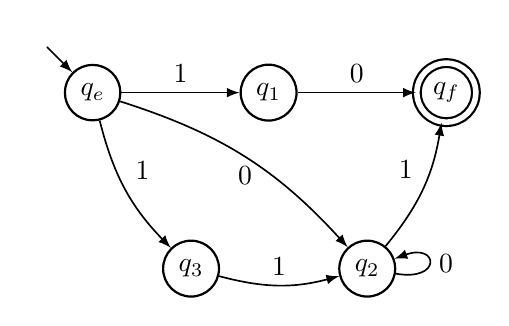
\begin{tikzpicture}[auto, >=latex, node distance=1.5cm, semithick]
  \node [state] (q1) {$q_1$};
  \node [state, starting, left=of q1] (qe) {$q_e$};
  \node [state, below=of qe, xshift=1.25cm] (q3) {$q_3$};
  \node [state, right=of q3] (q2) {$q_2$};
  \node [accepting, right=of q1] (qf) {$q_f$};

  \path[->] (qe) edge node [above] {$1$} (q1);
  \path[->] (q1) edge node [above] {$0$} (qf);

  \path[->] (qe) edge [bend left=15] node [below] {$0$} (q2);
  \path[->] (qe) edge [bend right=15] node {$1$} (q3);
  \path[->] (q3) edge [bend right=15] node {$1$} (q2);

  \path[->] (q2) edge [loop, out=-10, in=20, looseness=8] node [right] {$0$} (q2);
  \path[->] (q2) edge [bend right=15] node {$1$} (qf);
\end{tikzpicture}
\end{center}

The resulting FA is non-deterministic because of the two transitions on $1$ from
$q_e$. We may turn it into a DFA by merging $q_1$ and $q_3$.

\begin{center}
\begin{tikzpicture}[auto, >=latex, node distance=1.5cm, semithick]
  \node [state, starting, left=of q1, yshift=-1.25cm] (qe) {$q_e$};
  \node [state] (q1) {$q_1$};
  \node [state, below=of q1] (q2) {$q_2$};
  \node [accepting, right=of q1, yshift=-1.25cm] (qf) {$q_f$};

  \path[->] (qe) edge node {$1$} (q1);
  \path[->] (q1) edge node {$0$} (qf);

  \path[->] (qe) edge node {$0$} (q2);
  \path[->] (q1) edge node [left] {$1$} (q2);

  \path[->] (q2) edge [loop, out=-30, in=0, looseness=8] node [right] {$0$} (q2);
  \path[->] (q2) edge node {$1$} (qf);
\end{tikzpicture}
\end{center}

From the above we may conclude that the DFA for $10 + (0 + 11) 0^{*} 1$ is the
quintuple $(\{0, 1\}, \{q_e, q_f, q_1, q_2\}, \{q_e\}, \delta, \{q_f\})$
where $\delta$ is the transition function shown in Table \ref{tab:delta_1}.

\begin{table}[H]
\centering
\begin{tabular}{@{}ccc@{}}
\toprule
      & 0     & 1     \\ \midrule
$q_e$ & $q_2$ & $q_1$ \\ \midrule
$q_1$ & $q_f$ & $q_2$ \\ \midrule
$q_2$ & $q_2$ & $q_f$ \\ \bottomrule
\end{tabular}
\caption{Transition function $\delta$.}
\label{tab:delta_1}
\end{table}

\section{Regular Expression $01[((10)^* + 111)^* + 0]^*1$}
% We first simplify the expression $01[((10)^* + 111)^* + 0]^*1$. Note that $(a^*
% + b)^*$ is equivalent to $(a + b)^*$ as both accept the same languages. Applying
% this twice we get $01[10 + 111 + 0]^*1$.

We begin by constructing an NFA for the expression $01[((10)^* + 111)^* + 0]^*1$
following similar procedure as above.

\begin{center}
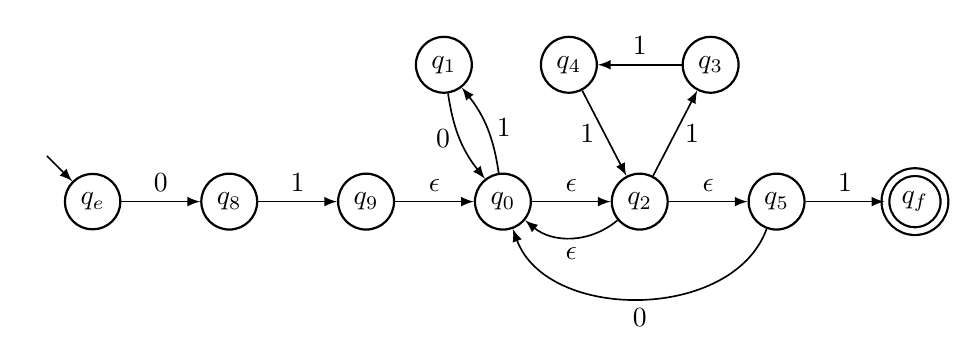
\begin{tikzpicture}[auto, >=latex, node distance=1cm, semithick]
  \node [state, starting] (qe) {$q_e$};
  \node [state, right=of qe] (q8) {$q_8$};
  \node [state, right=of q8] (q9) {$q_9$};
  \node [state, right=of q9] (q0) {$q_0$};
  \node [state, right=of q0] (q2) {$q_2$};
  \node [state, right=of q2] (q5) {$q_5$};
  \node [state, above=of q0, xshift=-0.75cm] (q1) {$q_1$};
  \node [state, above=of q2, xshift=0.9cm] (q3) {$q_3$};
  \node [state, above=of q2, xshift=-0.9cm] (q4) {$q_4$};
  \node [accepting, right=of q5] (qf) {$q_f$};

  \path[->] (qe) edge node {$0$} (q8);
  \path[->] (q8) edge node {$1$} (q9);
  \path[->] (q9) edge node {$\epsilon$} (q0);
  \path[->] (q0) edge node {$\epsilon$} (q2);
  \path[->] (q2) edge node {$\epsilon$} (q5);
  \path[->] (q5) edge node {$1$} (qf);

  \path[->] (q0) edge [bend right=15] node [right] {$1$} (q1);
  \path[->] (q1) edge [bend right=15] node [left] {$0$} (q0);

  \path[->] (q2) edge node [right] {$1$} (q3);
  \path[->] (q3) edge node [above] {$1$} (q4);
  \path[->] (q4) edge node [left] {$1$} (q2);

  \path[->] (q2) edge [bend left=40] node {$\epsilon$} (q0);
  \path[->] (q5) edge [bend left=70] node {$0$} (q0);
\end{tikzpicture}
\end{center}

We then transform this to a DFA by repeatedly applying the procedure of finding
the set of states for a given transition and computing the $\epsilon$ closure of
that set. Missing transitions are implicitly assumed to be going into the trap
state $\emptyset$.

\begin{center}
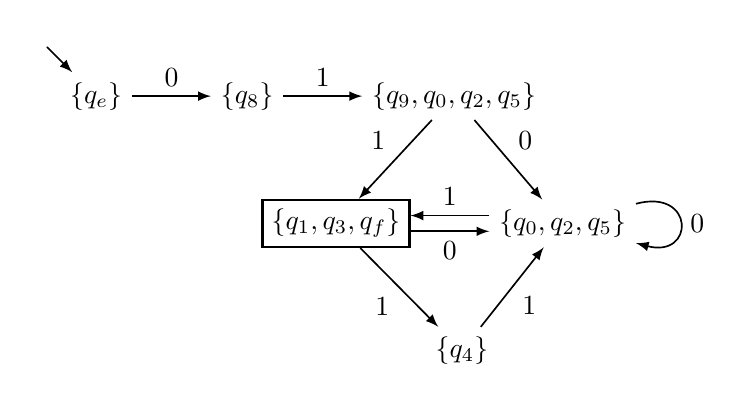
\begin{tikzpicture}[auto, >=latex, node distance=1cm, semithick]
  \node [set, starting] (qe) {$\{q_e\}$};
  \node [set, right=of qe] (q8) {$\{q_8\}$};
  \node [set, right=of q8] (q9025) {$\{q_9, q_0, q_2, q_5\}$};
  \node [acceptingset, below=of q9025, xshift=-1.5cm] (q13f) {$\{q_1, q_3, q_f\}$};
  \node [set, below=of q13f, xshift=1.6cm] (q4) {$\{q_4\}$};
  \node [set, right=of q13f] (q025) {$\{q_0, q_2, q_5\}$};

  \path[->] (qe) edge node {$0$} (q8);
  \path[->] (q8) edge node {$1$} (q9025);

  \path[->] (q9025) edge node [above left] {$1$} (q13f);
  \path[->] (q9025) edge node [above right] {$0$} (q025);

  \path[->] (q13f) edge node [below left] {$1$} (q4);
  \path[->] (q4) edge node [below right] {$1$} (q025);

  \path[->, transform canvas={yshift=-1mm}] (q13f) edge node [below] {$0$} (q025);
  \path[->, transform canvas={yshift=1mm}] (q025) edge node [above] {$1$} (q13f);

  \path[->] (q025) edge [loop right, looseness=4] node {$0$} (q025);
\end{tikzpicture}
\end{center}

The DFA has a single accpeting state marked with a rectangular outline. Renaming
the states we obtain

\begin{center}
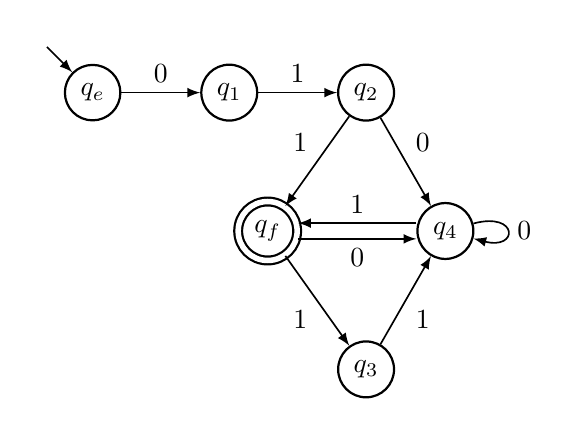
\begin{tikzpicture}[auto, >=latex, node distance=1cm, semithick]
  \node [state, starting] (qe) {$q_e$};
  \node [state, right=of qe] (q1) {$q_1$};
  \node [state, right=of q1] (q2) {$q_2$};
  \node [accepting, below=of q2, xshift=-1.25cm] (qf) {$q_f$};
  \node [state, below=of qf, xshift=1.25cm] (q3) {$q_3$};
  \node [state, right=of qf, xshift=0.5cm] (q4) {$q_4$};

  \path[->] (qe) edge node {$0$} (q1);
  \path[->] (q1) edge node {$1$} (q2);

  \path[->] (q2) edge node [above left] {$1$} (qf);
  \path[->] (q2) edge node [above right] {$0$} (q4);

  \path[->, transform canvas={yshift=-1mm}] (qf) edge node [below] {$0$} (q4);
  \path[->, transform canvas={yshift=1mm}] (q4) edge node [above] {$1$} (qf);

  \path[->] (qf) edge node [below left] {$1$} (q3);
  \path[->] (q3) edge node [below right] {$1$} (q4);

  \path[->] (q4) edge [loop right, looseness=8] node {$0$} (q4);
\end{tikzpicture}
\end{center}

Hence the DFA for $01[((10)^* + 111)^* + 0]^*1$ is the quintuple
$$
(\{0, 1\}, \{q_e, q_f, q_1, q_2, q_3, q_4\}, \{q_e\}, \delta, \{q_f\})
$$
where $\delta$ is the transition function shown in Table \ref{tab:delta_2}.

\begin{table}[H]
\centering
\begin{tabular}{@{}ccc@{}}
\toprule
      & 0           & 1     \\ \midrule
$q_e$ & $q_1$       & $\emptyset$ \\ \midrule
$q_1$ & $\emptyset$ & $q_2$ \\ \midrule
$q_2$ & $q_5$       & $q_f$ \\ \midrule
$q_3$ & $\emptyset$ & $q_4$ \\ \midrule
$q_4$ & $q_4$ & $q_f$ \\ \midrule
$q_f$ & $q_4$ & $q_3$ \\ \bottomrule
\end{tabular}
\caption{Transition function $\delta$.}
\label{tab:delta_2}
\end{table}

\section{Regular Expression $((0 + 1)(0 + 1))^* + ((0 + 1)(0 + 1)(0 + 1))^*$}
We begin by constructing an NFA for the expression $((0 + 1)(0 + 1))^* + ((0 +
1)(0 + 1)(0 + 1))^*$ identically as before.
\begin{center}
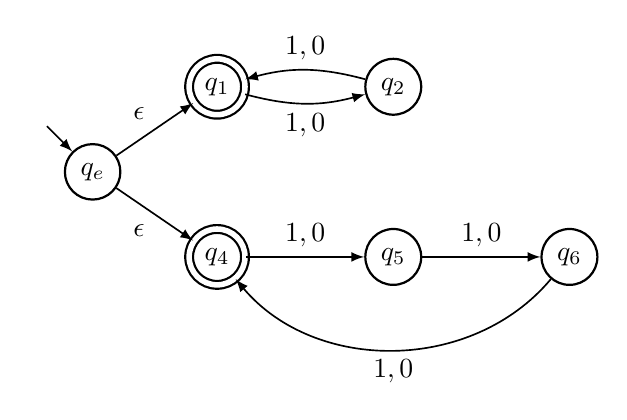
\begin{tikzpicture}[auto, >=latex, node distance=1.5cm, semithick]
  \node [state, starting] (qe) {$q_e$};
  \node [accepting, above right=of qe, yshift=-0.5cm] (q1f) {$q_1$};
  \node [state, right=of q1f] (q2) {$q_2$};
  \node [accepting, below right=of qe, yshift=0.5cm] (q4f) {$q_4$};
  \node [state, right=of q4f] (q5) {$q_5$};
  \node [state, right=of q5] (q6) {$q_6$};

  \path[->] (qe) edge node [above left] {$\epsilon$} (q1f);
  \path[->] (qe) edge node [below left] {$\epsilon$} (q4f);

  \path[->] (q1f) edge [bend right=15] node [below] {$1,0$} (q2);
  \path[->] (q2) edge [bend right=15] node [above] {$1,0$} (q1f);

  \path[->] (q4f) edge node {$1,0$} (q5);
  \path[->] (q5) edge node {$1,0$} (q6);
  \path[->] (q6) edge [bend left=50] node {$1,0$} (q4f);
\end{tikzpicture}
\end{center}

We then transform this to a DFA. Missing transitions are implicitly assumed to
be going into the trap state $\emptyset$.

\begin{center}
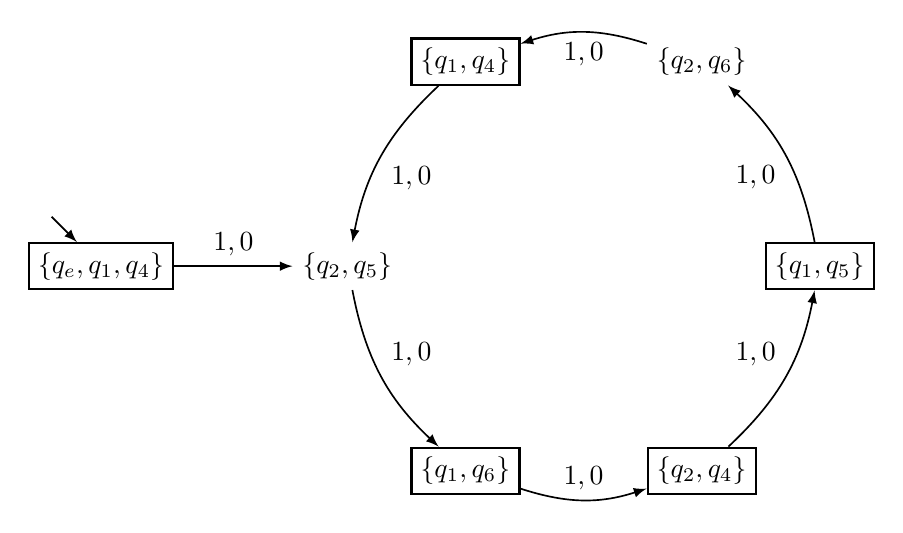
\begin{tikzpicture}[auto, >=latex, node distance=1.5cm, semithick]
  \node [set] (q25) at (180:3cm) {$\{q_2, q_5\}$};
  \node [acceptingset] (q16) at (240:3cm) {$\{q_1, q_6\}$};
  \node [acceptingset] (q24) at (300:3cm) {$\{q_2, q_4\}$};
  \node [acceptingset] (q15) at (0:3cm) {$\{q_1, q_5\}$};
  \node [set] (q26) at(60:3cm) {$\{q_2, q_6\}$};
  \node [acceptingset] (q14) at (120:3cm) {$\{q_1, q_4\}$};
  \node [acceptingset, starting, left=of q25] (qe14) {$\{q_e, q_1, q_4\}$};

  \path[->] (qe14) edge node {$1,0$} (q25);
  \path[->] (q25) edge [bend right=18] node {$1,0$} (q16);
  \path[->] (q16) edge [bend right=18] node {$1,0$} (q24);
  \path[->] (q24) edge [bend right=18] node {$1,0$} (q15);
  \path[->] (q15) edge [bend right=18] node {$1,0$} (q26);
  \path[->] (q26) edge [bend right=18] node {$1,0$} (q14);
  \path[->] (q14) edge [bend right=18] node {$1,0$} (q25);
\end{tikzpicture}
\end{center}

The resulting DFA has multiple accepting states marked with rectangular
outlines. Renaming the states we obtain

\begin{center}
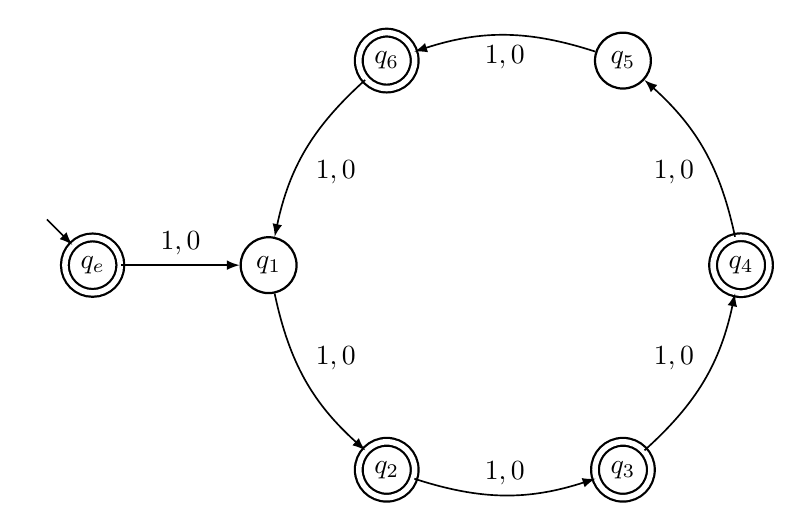
\begin{tikzpicture}[auto, >=latex, node distance=1.5cm, semithick]
  \node [state] (q1) at (180:3cm) {$q_1$};
  \node [accepting] (q2) at (240:3cm) {$q_2$};
  \node [accepting] (q3) at (300:3cm) {$q_3$};
  \node [accepting] (q4) at (0:3cm) {$q_4$};
  \node [state] (q5) at(60:3cm) {$q_5$};
  \node [accepting] (q6) at (120:3cm) {$q_6$};
  \node [accepting, starting, left=of q1] (qe) {$q_e$};

  \path[->] (qe) edge node {$1,0$} (q1);
  \path[->] (q1) edge [bend right=18] node {$1,0$} (q2);
  \path[->] (q2) edge [bend right=18] node {$1,0$} (q3);
  \path[->] (q3) edge [bend right=18] node {$1,0$} (q4);
  \path[->] (q4) edge [bend right=18] node {$1,0$} (q5);
  \path[->] (q5) edge [bend right=18] node {$1,0$} (q6);
  \path[->] (q6) edge [bend right=18] node {$1,0$} (q1);
\end{tikzpicture}
\end{center}

We note that the state $q_e$ is reduntant as the state $q_6$ is equivalent to it
(accepting state, identical transition function). Thus we may remove $q_e$ and
make $q_6$ the entry state (and also rename it to $q_e$).

\begin{center}
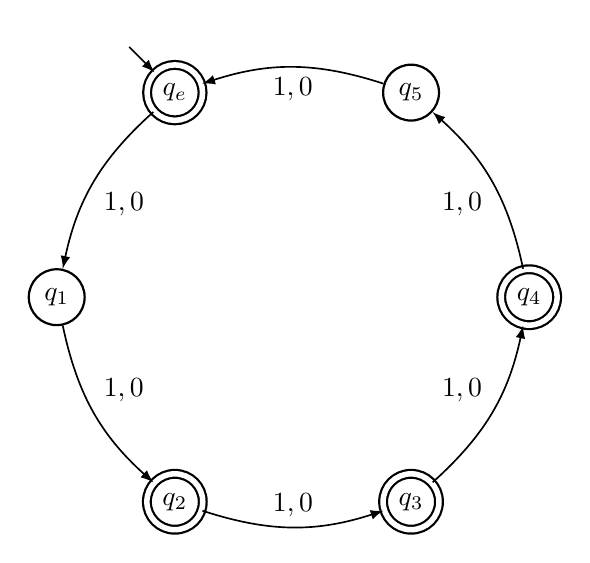
\begin{tikzpicture}[auto, >=latex, node distance=1.5cm, semithick]
  \node [state] (q1) at (180:3cm) {$q_1$};
  \node [accepting] (q2) at (240:3cm) {$q_2$};
  \node [accepting] (q3) at (300:3cm) {$q_3$};
  \node [accepting] (q4) at (0:3cm) {$q_4$};
  \node [state] (q5) at(60:3cm) {$q_5$};
  \node [accepting, starting] (qe) at (120:3cm) {$q_e$};

  \path[->] (q1) edge [bend right=18] node {$1,0$} (q2);
  \path[->] (q2) edge [bend right=18] node {$1,0$} (q3);
  \path[->] (q3) edge [bend right=18] node {$1,0$} (q4);
  \path[->] (q4) edge [bend right=18] node {$1,0$} (q5);
  \path[->] (q5) edge [bend right=18] node {$1,0$} (qe);
  \path[->] (qe) edge [bend right=18] node {$1,0$} (q1);
\end{tikzpicture}
\end{center}

The final DFA for $((0 + 1)(0 + 1))^* + ((0 + 1)(0 + 1)(0 + 1))^*$ is the
quintuple
$$
(\{0, 1\}, \{q_e, q_f, q_1, q_2, q_3, q_4, q_5\}, \{q_e\}, \delta, \{q_e,
q_2, q_3, q_4\})
$$
where $\delta$ is the transition function shown in Table \ref{tab:delta_3}.

\begin{table}[H]
\centering
\begin{tabular}{@{}ccc@{}}
\toprule
      & 0     & 1     \\ \midrule
$q_1$ & $q_2$ & $q_2$ \\ \midrule
$q_2$ & $q_3$ & $q_3$ \\ \midrule
$q_3$ & $q_4$ & $q_4$ \\ \midrule
$q_4$ & $q_5$ & $q_5$ \\ \midrule
$q_5$ & $q_6$ & $q_6$ \\ \midrule
$q_e$ & $q_1$ & $q_1$ \\ \midrule
\end{tabular}
\caption{Transition function $\delta$.}
\label{tab:delta_3}
\end{table}

\end{document}
